\typeout{IJCAI-16 Instructions for Authors}
%DIF LATEXDIFF DIFFERENCE FILE
%DIF DEL /u/jesse/Downloads/paper/ijcai16.tex   Tue Feb  2 19:32:15 2016
%DIF ADD ijcai16.tex                            Tue Apr  5 23:07:18 2016

\documentclass{article}
% The file ijcai16.sty is the style file for IJCAI-16 (same as ijcai07.sty).
\usepackage{ijcai16}

% Use the postscript times font!
\usepackage{times}

% the following package is optional:
%\usepackage{latexsym} 

% author added packages
\usepackage{xspace}
\usepackage{graphicx}
\usepackage{epsfig}
\usepackage{array}

\newcommand{\ispy}{``I Spy''\xspace}
\newcommand{\examplepicsize}{0.125}
\newcommand{\pictablew}{0.4in}

%\title{Grounded Attribute Learning with Multi-Modal Perception}
\title{Learning Multi-Modal Grounded Linguistic Semantics by Playing \ispy}
\author{\DIFdelbegin \DIFdel{Paper XXX}\DIFdelend \DIFaddbegin \DIFadd{Jesse Thomason, Jivko Sinapov, Maxwell Svetlik, Peter Stone,}\and \DIFadd{Raymond Mooney }\\
\DIFadd{Department of Computer Science, University of Texas at Austin}\\
\DIFadd{Austin, TX 78712, USA}\\
\{\DIFadd{jesse, jsinapov, maxwell, pstone, mooney}\}\DIFadd{@cs.utexas.edu}\DIFaddend }
%DIF < %\author{name \\ 
%DIF < %affiliation  \\
%DIF < %email}
%DIF PREAMBLE EXTENSION ADDED BY LATEXDIFF
%DIF UNDERLINE PREAMBLE %DIF PREAMBLE
\RequirePackage[normalem]{ulem} %DIF PREAMBLE
\RequirePackage{color}\definecolor{RED}{rgb}{1,0,0}\definecolor{BLUE}{rgb}{0,0,1} %DIF PREAMBLE
\providecommand{\DIFadd}[1]{{\protect\color{blue}\uwave{#1}}} %DIF PREAMBLE
\providecommand{\DIFdel}[1]{{\protect\color{red}\sout{#1}}}                      %DIF PREAMBLE
%DIF SAFE PREAMBLE %DIF PREAMBLE
\providecommand{\DIFaddbegin}{} %DIF PREAMBLE
\providecommand{\DIFaddend}{} %DIF PREAMBLE
\providecommand{\DIFdelbegin}{} %DIF PREAMBLE
\providecommand{\DIFdelend}{} %DIF PREAMBLE
%DIF FLOATSAFE PREAMBLE %DIF PREAMBLE
\providecommand{\DIFaddFL}[1]{\DIFadd{#1}} %DIF PREAMBLE
\providecommand{\DIFdelFL}[1]{\DIFdel{#1}} %DIF PREAMBLE
\providecommand{\DIFaddbeginFL}{} %DIF PREAMBLE
\providecommand{\DIFaddendFL}{} %DIF PREAMBLE
\providecommand{\DIFdelbeginFL}{} %DIF PREAMBLE
\providecommand{\DIFdelendFL}{} %DIF PREAMBLE
%DIF END PREAMBLE EXTENSION ADDED BY LATEXDIFF

\begin{document}

\maketitle

\begin{abstract}
% The abstract should be no more than 200 words long
Grounded language learning bridges words like `red' and `square' with robot perception.
The vast majority of existing work in this space limits robot perception to vision.
In this paper, we build perceptual models that use haptic, auditory, and proprioceptive data acquired through robot exploratory behaviors to go beyond vision.
Our system learns to ground natural language words describing objects using supervision from an interactive human-robot \ispy game.
In this game, the human and robot take turns describing one object among several, then trying to guess which object the other has described.
All supervision labels were gathered from human participants physically present to play this game with a robot.
We demonstrate that our multi-modal system for grounding natural language outperforms a traditional, vision-only grounding framework by comparing the two on the \ispy task.
We also provide a qualitative analysis of the groundings learned in the game, visualizing what words are understood better with multi-modal sensory information as well as identifying learned word meanings that correlate with physical object properties (e.g. `\DIFdelbegin \DIFdel{empty}\DIFdelend \DIFaddbegin \DIFadd{small}\DIFaddend ' negatively correlates with object weight).
\end{abstract}

\section{Introduction}
\label{sec:introduction}
Robots need to be able to connect language to their environment in order to discuss real world objects with humans.
Mapping from referring expressions such as ``the blue cup'' to an object referent in the world is an example of the \textit{symbol grounding problem}~\cite{harnad:phys90}.
Symbol grounding involves connecting internal representations of information in a machine to real world data from its sensory perception.
\textit{Grounded language learning} bridges these symbols with natural language.

Early work on grounded language learning enabled a machine to map from adjectives and nouns such as ``red'' and ``block'' to objects in a scene through vision-based classifiers~\cite{roy:evocomm01}.
We refer to adjectives and nouns that describe properties of objects as language \textit{predicates}.
Most work has focused on grounding predicates through visual information. However, other sensory modalities such as haptic and auditory are also useful in allowing robots to discriminate between object categories~\cite{sinapov:icra14}.
This paper explores grounding language predicates by considering visual, haptic, auditory, and proprioceptive senses. 

A home or office robot can explore objects in an unsupervised way to gather perceptual data, but needs human supervision to connect this data to language.
Learning grounded semantics through human-robot dialog allows a system to acquire the relevant knowledge without the need for laborious labeling of numerous objects for every potential lexical descriptor.
A few groups have explored learning from interactive linguistic games such as \ispy and ``20 Questions'' \cite{parde:ijcai15,vogel:aaai10}; however, these studies only employed vision (see Section \ref{sec:relatedwork}).

\begin{figure}
\centering
\begin{tabular}{cc}
	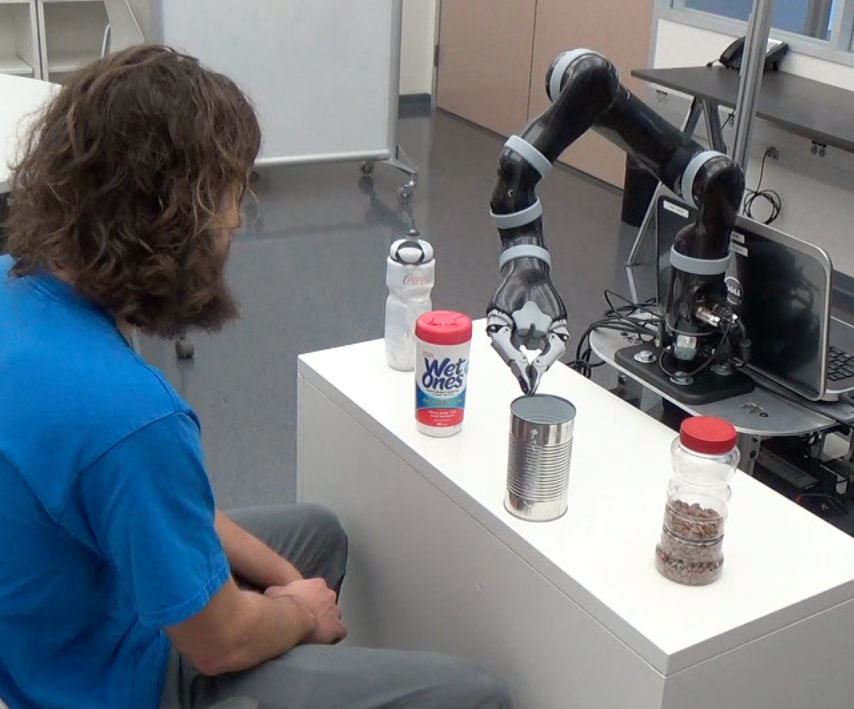
\includegraphics[width=0.225\textwidth]{figures/silver_round_and_empty_cropped.png} &
	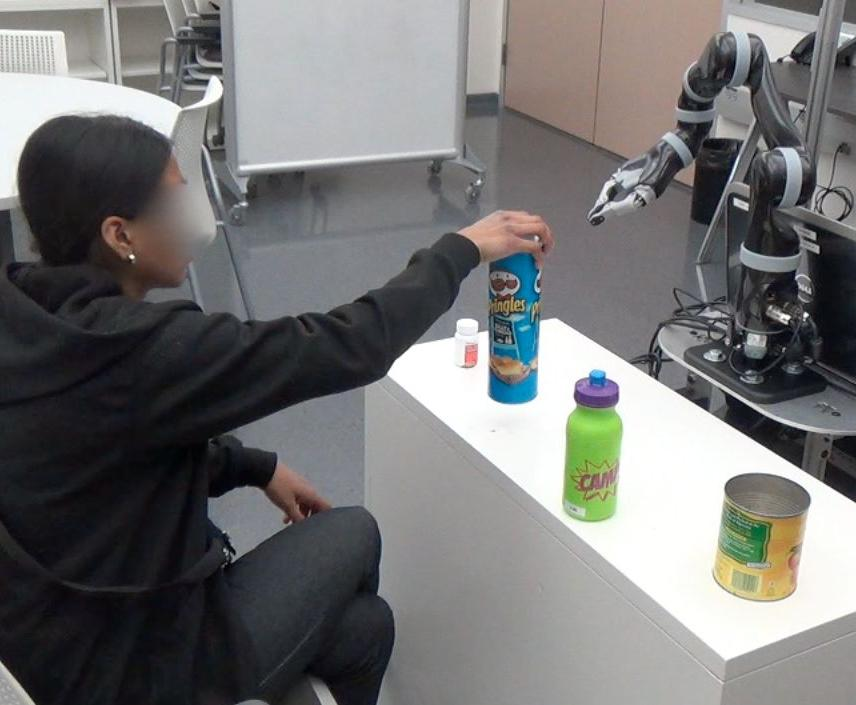
\includegraphics[width=0.225\textwidth]{figures/light_tall_tub_cropped.jpg} \\
\end{tabular}
\caption{\textbf{Left}: the robot guesses an object described by a human participant as ``silver, round, and empty.'' \textbf{Right}: a human participant guesses an object described by the robot as ``light,'' ``tall,'' and ``tub.''}
\label{fig:ispy}
\end{figure}

We use a variation on the children's game \ispy, as a learning framework for gathering human language labels for objects to learn multi-modal grounded lexical semantics (Figure~\ref{fig:ispy}).
Our experimental results test generalization to new objects not seen during training and illustrate both that the system learns accurate word meanings and that modalities beyond vision improve its performance.

To our knowledge, this is the first robotic system to perform natural language grounding using multi-modal sensory perception through feedback with human users.

\section{Related Work}
\label{sec:relatedwork}
% relation to grounded language learning tasks
Researchers have made substantial progress on grounding language for robots, enabling tasks such as object recognition and route following from verbal descriptions.
Early work used vision together with speech descriptions of objects to learn grounded semantics~\cite{roy:cogsci02}.

In the past few years, much of this work has focused on combining language with visual information.
For grounding referring expressions in an environment, many learn perceptual classifiers for words given some pairing of human descriptions and labeled scenes~\cite{liu:acl14,malinowski:nips14,mohan:acs13,sun:icra13,dindo:iros10,vogel:aaai10}.
Some approaches additionally incorporate language models into the learning phase~\cite{spranger:ijcai15,krishnamurthy:acl13,perera:aaai13,matuszek:icml12}.
Incorporating a language model also allows for more robust generation of robot referring expressions for objects, as explored in~\cite{tellex:rss14}.
\DIFdelbegin \DIFdel{Our }\DIFdelend \DIFaddbegin \DIFadd{In general, referring expression generation is difficult in dialog~\mbox{%DIFAUXCMD
\cite{fang:aaai14}
}%DIFAUXCMD
.
Since we are focused on comparing multi-modal to vision-only grounding, our }\DIFaddend method uses simple language understanding and constructs new predicate classifiers for each unseen content word used by a human playing \ispy, and our \DIFaddbegin \DIFadd{basic }\DIFaddend generation system for describing objects is based only on these predicate classifiers.

Outside of robotics, there has been some work on combining language with sensory modalities other than vision, such as audio~\cite{kiela:emnlp15}.
Unlike that line of work, our system is embodied in a learning robot that manipulates objects to gain non-visual sensory experience.

Including a human in the learning loop provides a more realistic learning scenario for applications such as household and office robotics.
Past work has used human speech plus gestures describing sets of objects on a table as supervision to learn attribute classifiers~\cite{matuszek:aaai14,kollar:rss13}. Recent work introduced the \ispy game as a supervisory framework for grounded language learning~\cite{parde:ijcai15}.
Our work differs from these by using additional sensory data beyond vision to build object attribute classifiers. Additionally, in our instantiation of the \ispy task, the robot and the human both take a turn describing objects, where in previous work~\cite{parde:ijcai15} only humans gave descriptions.


\section{Dataset}
\label{sec:dataset}
\begin{figure}
\centering
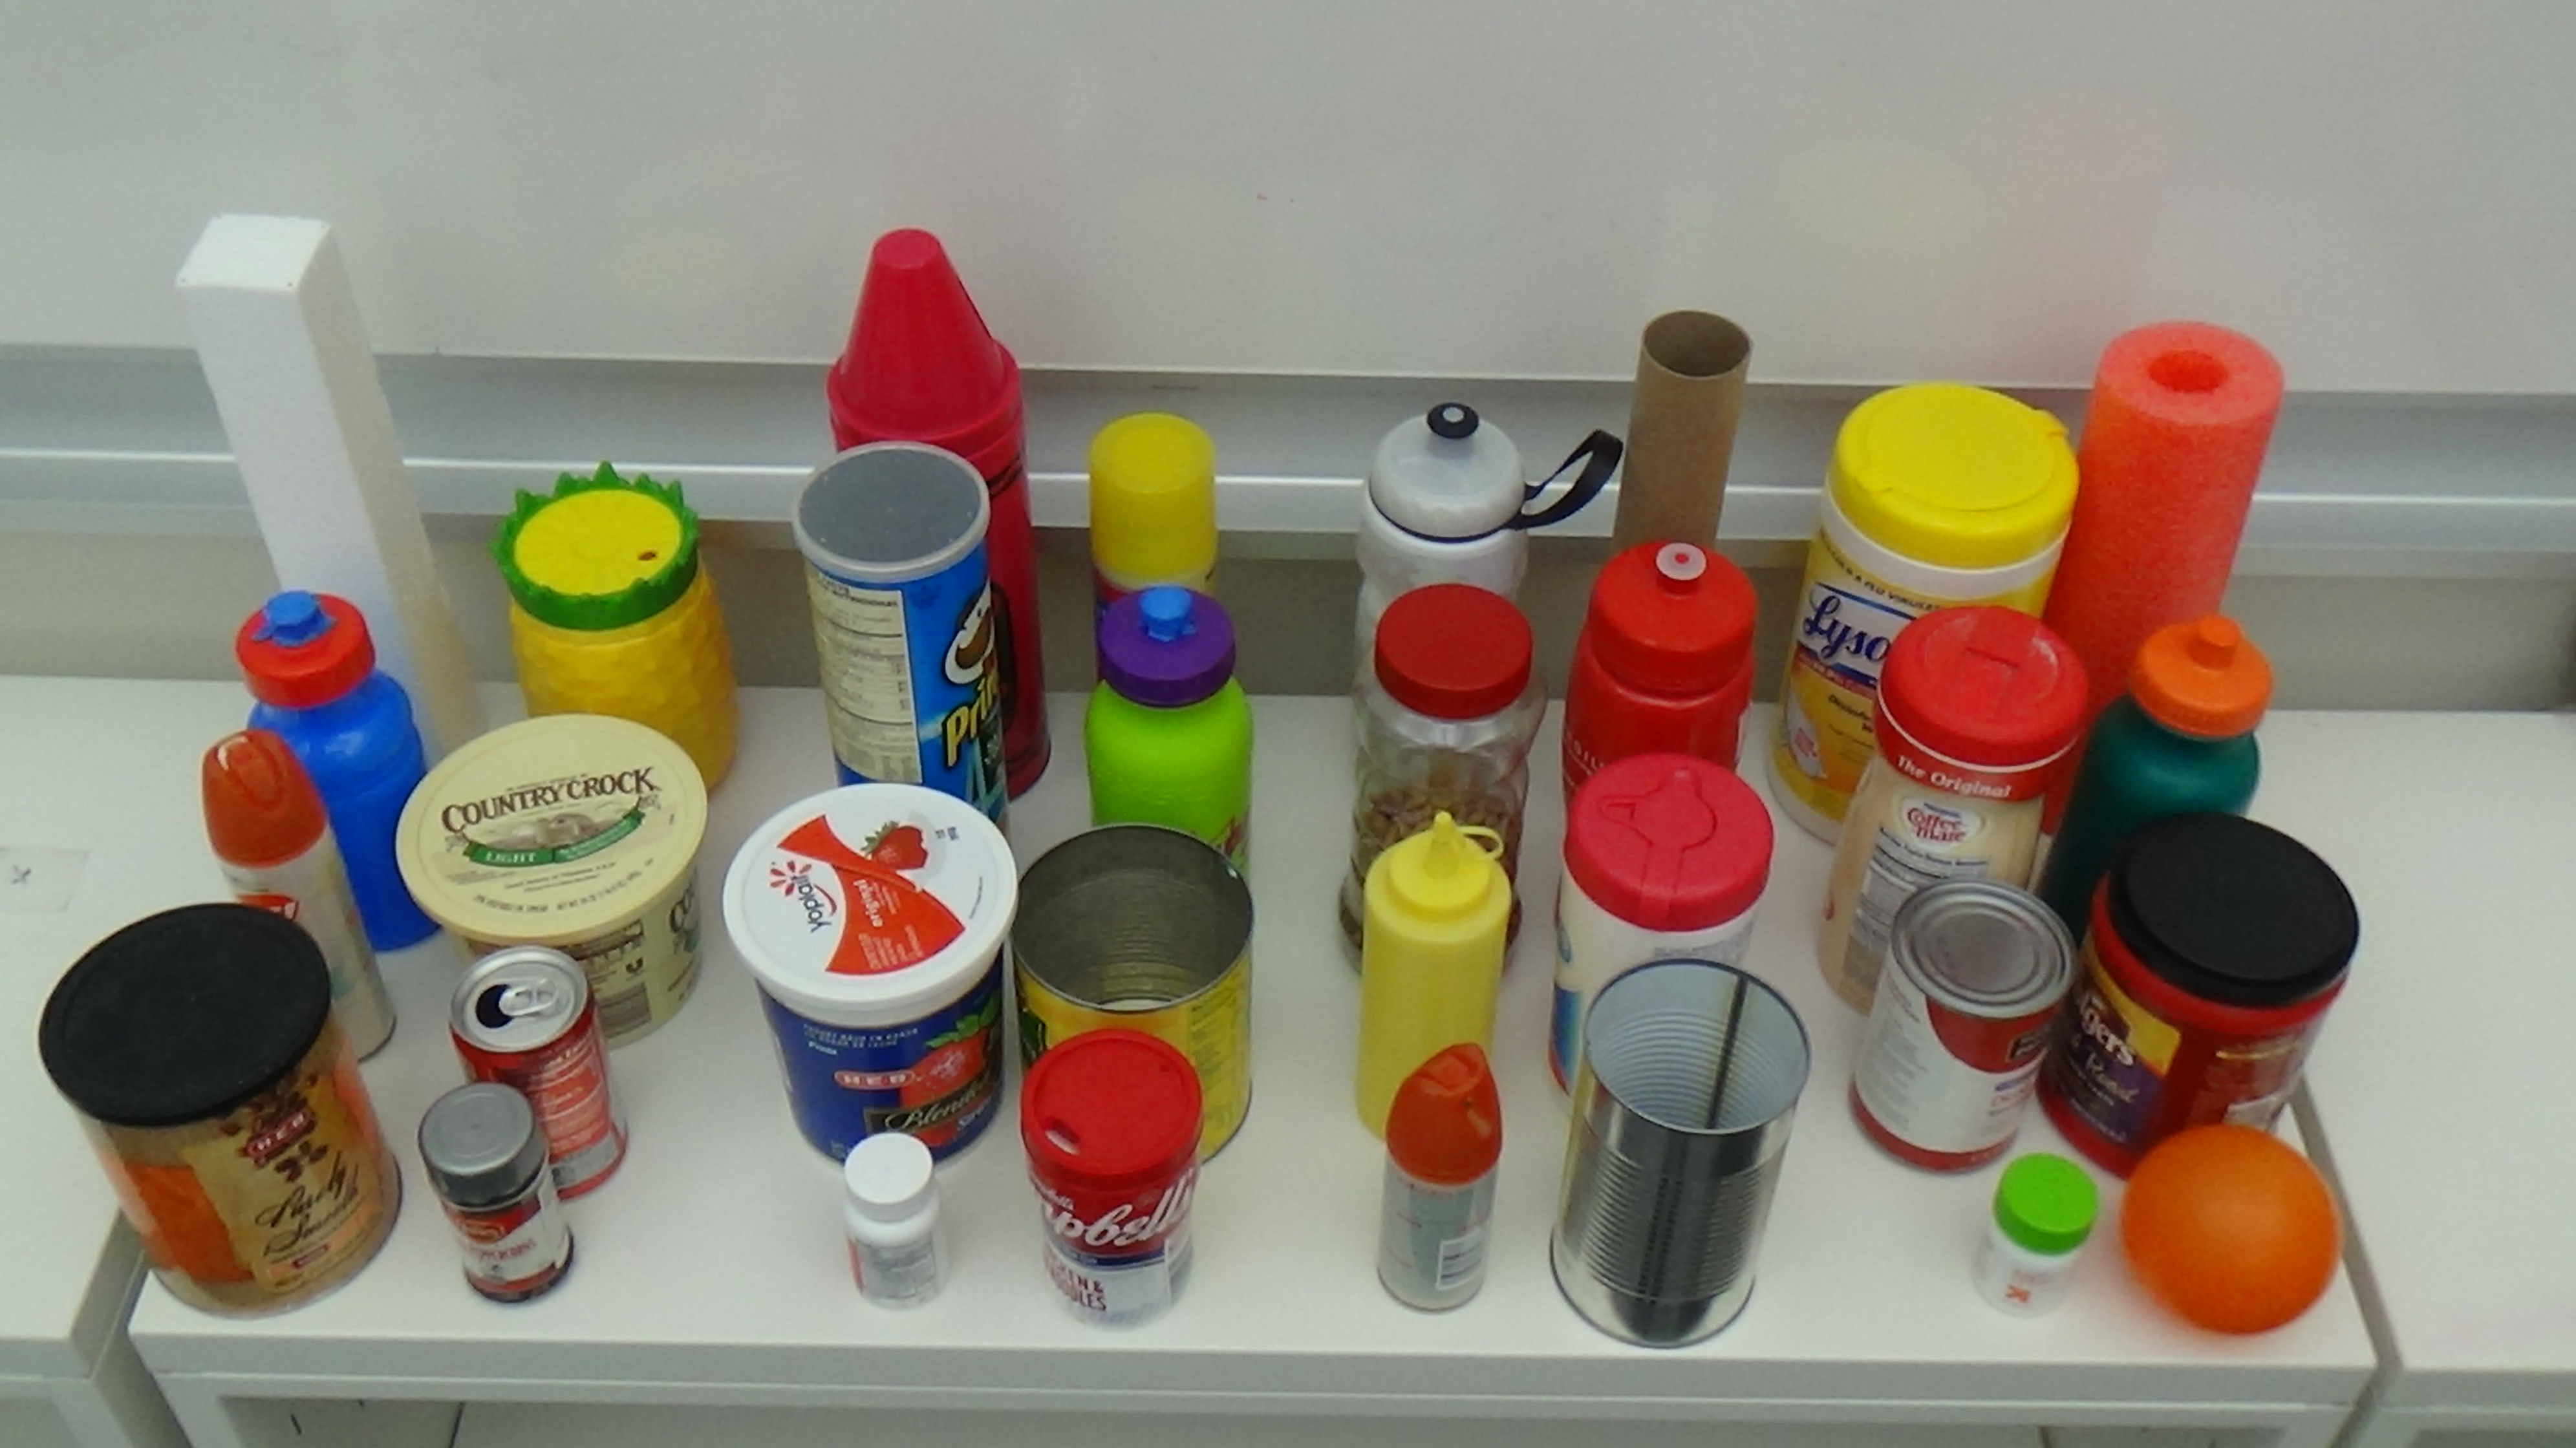
\includegraphics[width=0.3\textwidth]{figures/objects.jpg}
\caption{Objects used in the \ispy game divided into the four folds discussed in Section~\ref{ssec:methodology}, from fold 0 on the left to fold 3 on the right.}
\label{fig:objects}
\end{figure}

The robot used in this study was a Kinova MICO arm mounted on top of a custom-built mobile base, which remained stationary during our experiment.
The robot's sensors included joint effort sensors in each of the robot arm's motors, a microphone mounted on the mobile base, and the Xtion ASUS Pro RGBD camera.
The set of objects used in this experiment consisted of 32 common household items including cups, bottles, cans, and other containers, shown in Figure~\ref{fig:objects}.
Some of the objects contained liquids or other contents (e.g., coffee beans) while others were empty.
\DIFaddbegin \DIFadd{Contemporary work gives a more detailed description of this object dataset~\mbox{%DIFAUXCMD
\cite{sinapov:ijcai16}
}%DIFAUXCMD
, but we briefly describe the exploration and modalities below.
}\DIFaddend 

\subsection{Exploratory Behaviors and Sensory Modalities}
\label{ssec:contexts}

\begin{center}
\begin{figure}[t]
\setlength{\unitlength}{1in}
 \centerline{
\begin{picture}(3.5,2.5)
\put(0.0,1.4){\psfig{file=figures/behaviors/grasp1.eps,width=1.1in}}
\put(0.4,1.275){grasp}
\put(1.2,1.4){\psfig{file=figures/behaviors/lift1_arrow.eps,width=1.1in}}
\put(1.7,1.275){lift}
\put(2.4,1.4){\psfig{file=figures/behaviors/lower1_arrow.eps,width=1.1in}}
\put(2.8,1.275){lower}
\put(0.0,0.075){\psfig{file=figures/behaviors/drop1.eps,width=1.1in}}
\put(0.45,-0.05){drop}
\put(1.2,0.075){\psfig{file=figures/behaviors/press1_arrow.eps,width=1.1in}}
\put(1.6,-0.05){press}
\put(2.4,0.075){\psfig{file=figures/behaviors/push2_arrow.eps,width=1.1in}}
\put(2.8,-0.05){push}
\end{picture}
}
\caption{The behaviors the robot used to explore the objects.
The arrows indicate the direction of motion of the end-effector for each behavior.
In addition, the {\it hold} behavior (not shown) was performed after the {\it lift} behavior by simply holding the object in place for half a second.}
\label{fig:behaviors}
\end{figure}
\end{center}
\vspace {-5mm}

Prior to the experiment, the robot explored the objects using the methodology described by Sinapov et al.~\shortcite{sinapov:ras14}, and the dimensionality of the raw auditory, haptic, and proprioceptive data were reduced comparably (final dimensionality given in Table~\ref{tab:feature_space_of_contexts}\DIFaddbegin \DIFadd{)}\DIFaddend .
In our case, the robot used 7 distinct actions: {\it grasp}, {\it lift}, {\it hold}, {\it lower}, {\it drop}, {\it push}, and {\it press}, shown in Figure~\ref{fig:behaviors}.
During the execution of each action, the robot recorded the sensory perceptions from {\it haptic} (i.e., joint efforts) and {\it auditory} sensory modalities.
During the {\it grasp} action, the robot recorded {\it proprioceptive} (i.e., joint angular positions) sensory information from its fingers.
The joint efforts and joint positions were recorded for all 6 joints at 15 Hz.
The auditory sensory modality was represented as the Discrete Fourier Transform computed using 65 frequency bins.

In addition to the 7 interactive behaviors, the robot also performed the {\it look} action prior to grasping the object which produced three different kinds of sensory modalities: 1) an RGB color histogram of the object using 8 bins per channel; 2) Fast point feature histogram ({\it fpfh}) shape features~\cite{rusu:icra09} as implemented in the Point Cloud Library~\cite{aldoma:ram12}; and 3) deep visual features from the 16-layer VGG network~\cite{simonyan:corr14}.
The first two types of features were computed using the segmented point cloud of the object while the deep features were computed using the 2D image of the object. 

\begin{table}
\centering
\begin{tabular}[h]{|l|c|c|c|}
	\hline
	\bf Behavior & \multicolumn{3}{c|}{\bf Modality} \\ \hline \hline
	& \bf color & \bf fpfh & \bf vgg \\ \hline
	\bf look & 64 & 308 & 4096 \\ \hline \hline
	& \bf audio & \bf haptics & \bf proprioception \\ \hline
	\bf grasp & 100 & 60 & 20 \\ \hline
	\bf drop, hold, & & & \\
	\bf lift, lower, & 100 & 60 & \\
	\bf press, push & & & \\ \hline
\end{tabular}
\caption{The number of features extracted from each \textit{context}, or combination of robot behavior and perceptual modality.}
\label{tab:feature_space_of_contexts}
\end{table}

Thus, each of the robot's 8 actions produced two to three different kinds of sensory signals.
Each viable combination of an action and a sensory modality is a unique sensorimotor context.
In our experiment, the set of contexts $\mathcal{C}$ was of size  $2 \times 3 + 6 \times 2 = 18$.
The robot performed its full sequence of exploratory actions on each object 5 different times (for the {\it look} behavior, the object was rotated to a new angle each time). Given a context $c \in \mathcal{C}$ and an object $i \in \mathcal{O}$, let the set $\mathcal{X}_i^c$ contain all five feature vectors observed with object $i$ in context $c$.
\DIFdelbegin \DIFdel{Table~\ref{tab:feature_space_of_contexts} gives the size of the feature vectors extracted for each context.
}\DIFdelend 

\section{Task Definition}
\label{sec:taskdefinition}
In our \ispy task\footnote{Video demonstrating the \ispy task and robot learning: \DIFdelbegin \texttt{\DIFdel{https://youtu.be/JdcmreKPC-k}}%DIFAUXCMD
\DIFdelend \DIFaddbegin \texttt{\DIFadd{https://youtu.be/jLHzRXPCi}\\\DIFadd{SUBSCRIPTNB}{\DIFadd{w}}}\DIFaddend }, the human and robot take turns describing objects from among 4 on a tabletop (Figure~\ref{fig:ispy}).
Participants were asked to describe objects using attributes.
As an example, we suggested participants describe an object as ``black rectangle'' as opposed to ``whiteboard eraser.''
Additionally, participants were told they could handle the objects physically before offering a description, but were not explicitly asked to use non-visual predicates.
Once participants offered a description, the robot guessed candidate objects in order of computed confidence (see Section~\ref{ssec:gll}) until one was confirmed correct.

In the second half of each round, the robot picked an object and then described it with up to three predicates (see Section~\ref{ssec:gll}).
The participant was again able to pick up and physically handle objects before guessing.
The robot confirmed or denied each participant guess until the correct object was chosen.

\ispy gameplay admits two metrics.
The \textbf{robot guess} metric is the number of turns the robot took to guess what object the participant was describing.
The \textbf{human guess} metric is the complement.
Using these metrics, we compare the performance of two \ispy playing systems (\textbf{multi-modal} and \textbf{vision-only}) as described in Section ~\ref{sec:experiment}.
We also compare the agreement between both systems' predicate classifiers and human labels acquired during the game.

\section{Implementation}
\label{sec:implementation}
To play \ispy, we first gathered sensory data from the set of objects through robot manipulation behaviors (described in Section~\ref{sec:dataset}).
When playing a game, the robot was given unique identifying numbers for each object on the table and could look up relevant feature vectors when performing grounding.

During the course of the game, the robot used its RGBD camera to detect the locations of the objects and subsequently detect whenever a human reached out and touched an object in response to the robot's turn.
The robot was also equipped with the ability to reach out and point to an object when it was the robot's turn to guess.
We implemented robot behaviors in the Robot Operating System\footnote{\texttt{http://www.ros.org/}} and performed text-to-speech using the Festival Speech Synthesis System\footnote{\texttt{http://www.cstr.ed.ac.uk/projects/festival/}}.

	\subsection{Multi-Modal Perception}
	\label{ssec:mmp}
For each language predicate $p$, a classifier $G_p$ was learned to decide whether objects possessed the attribute denoted by $p$.
This classifier was informed by context sub-classifiers that determined whether $p$ held for subsets of an object's features.

The feature space of objects was partitioned by context, as discussed in Section~\ref{ssec:contexts}.
Each context classifier $M_{c}, c\in\mathcal{C}$ was a quadratic-kernel SVM trained with positive- and negative-labels for context feature vectors derived from the \ispy game (Section~\ref{ssec:gll}).
We defined $M_{c}(\mathcal{X}_i^c)\in [-1,1]$ as the average classifier output over all observations for object $i\in\mathcal{O}$ (individual SVM decisions on observations were in $\{-1,1\}$).

Following previous work in multi-modal exploration~\cite{sinapov:icra14}, for each context we calculated Cohen's Kappa $\kappa_{c}\in[0,1]$ to measure the agreement across observations between the decisions of the $M_{c}$ classifier and the ground truth labels from the \ispy game\footnote{We use $\kappa$ instead of accuracy because it better handles skewed-class data than accuracy, which could be deceptively high for a classifier that always returns false for a low-frequency predicate. We round negative $\kappa$ up to $0$.}.
Given these context classifiers and associated $\kappa$ confidences, we calculate an overall decision, $G_p(i)$, for $i\in\mathcal{O}$ for each behavior $b$ and modality $m$ as:
\begin{equation}
	G_p(i) = \sum_{c\in\mathcal{C}}{\kappa_{c} M_{c}(\mathcal{X}_i^c)} \in [-1,1]
\end{equation}
The sign of $G_p(i)$ gives a decision on whether $p$ applies to $i$ with confidence $|G_p(i)|$.

For example, the final classifier built for `fat'$\in P$ gives $G_{\texttt{fat}}(\texttt{wide-yellow-cylinder}) = 0.137$, a positive classification, with $\kappa_{gr,au}=0.515$ for the \textit{gr}asp behavior's \textit{au}ditory modality, the most confident context. This context may be useful for this predicate because the sound of the fingers' motors would stop sooner for wider objects.

	\subsection{Grounded Language Learning}
	\label{ssec:gll}
Language predicates and their positive/negative object labels were gathered through human-robot dialog during the \ispy game.
The human participant and robot were seated at opposite ends of a small table.
A set of 4 objects were placed on the table for both to see (Figure~\ref{fig:ispy}).
We denote the set of objects on the table during a given game $\mathcal{O}_T$.

\textbf{Human Turn.} On the participant's turn, the robot asked him or her to pick an object and describe it in one phrase.
We used a standard stopword list to strip out non-content words from the participant's description.
The remaining words were treated as a set of language predicates, $\mathcal{H}_p$.
The robot assigned scores $S$ to each object $i\in \mathcal{O}_T$ on the table.
\begin{equation}
	S(i) = \sum_{p\in \mathcal{H}_p}{G_p(i)}
\end{equation}
The robot guessed objects in descending order by score (ties broken randomly) by pointing at them and asking whether it was correct.
When the correct object was found, it was added as a positive training example for all predicates $p\in \mathcal{H}_p$ for use in future training.

\textbf{Robot Turn.} On the robot's turn, an object was chosen at random from those on the table.
To describe the object, the robot scored the set of known predicates learned from previous play.
Following Gricean principles~\cite{grice:bkchapter75}, the robot attempted to describe the object with predicates that applied but did not ambiguously refer to other objects.
We used a predicate score $R$ that rewarded describing the chosen object $i^*$ and penalized describing the other objects on the table.
\begin{equation}
	R(p) = |O_T|G_p(i^*) - \sum_{j\in{\mathcal{O}_T}\setminus\{i^*\}}{G_p(j)}
\end{equation}
The robot choose up to three highest scoring predicates $\hat{P}$ to describe object $i^*$, using fewer if $S<0$ for those remaining.
Once ready to guess, the participant touched objects until the robot confirmed that they had guessed the right one ($i^*$).

The robot then pointed to $i^*$ and engaged the user in a brief follow-up dialog in order to gather both positive and negative labels for $i^*$.
In addition to predicates $\hat{P}$ used to describe the object, the robot selected up to $5-|\hat{P}|$ additional predicates $\bar{P}$.
$\bar{P}$ were selected randomly with $p\in P\setminus\hat{P}$ having a chance of inclusion proportional to $1-|G_p(i^*)|$, such that classifiers with low confidence in whether or not $p$ applied to $i^*$ were more likely to be selected.
The robot then asked the participant whether they would describe the object $i^*$ using each $p\in\hat{P}\cup\bar{P}$.
Responses to these questions provided additional positive/negative labels on object $i^*$ for these predicates for use in future training.


\section{Experiment}
\label{sec:experiment}
To determine whether multi-modal perception helps a robot learn grounded language, we had two different systems play \ispy with 42 human participants.
The baseline \textbf{vision only} system used only the \textit{look} behavior when grounding language predicates, analogous to many past works as discussed in Section~\ref{sec:relatedwork}.
Our \textbf{multi-modal} system used the full suite of behaviors and associated haptic, proprioceptive, and auditory modalities shown in Table~\ref{tab:feature_space_of_contexts} when grounding language predicates.

	\subsection{Methodology}
	\label{ssec:methodology}
\textbf{Data Folds.}
We divided our 32-object dataset into 4 folds.
For each fold, at least 10 human participants played \ispy with both the \textbf{vision only} and \textbf{multi-modal} systems (12 participants in the final fold).
Four games were played by each participant.
The \textbf{vision only} system and \textbf{multi-modal} system were each used in 2 games, and these games' temporal order was randomized.
Each system played with all 8 objects per fold, but the split into 2 groups of 4 and the order of objects on the table were randomized.

For fold 0, the systems were undifferentiated and so only one set of 2 games was played by each participant. 
For subsequent folds, the systems were incrementally trained using labels from previous folds only, such that the systems were always being tested against novel, unseen objects.
This contrasts prior work using the \ispy game~\cite{parde:ijcai15}, where the same objects were used during training and testing.

\textbf{Human Participants.} Our 42 participants were undergraduate and graduate students as well as some staff at our university.

At the beginning of each trial, participants were shown an instructional video of one of the authors playing a single game of \ispy with the robot, then given a sheet of instructions about the game and how to communicate with the robot. 
In every game, participants took one turn and the robot took one turn.

To avoid noise from automatic speech recognition, a study coordinator remained in the room and transcribed the participant's speech to the robot from a remote computer.
This was done discretely and not revealed to the participant until debriefing when the games were over.


	\subsection{Quantitative Results}
	\label{ssec:results}
To determine whether our \textbf{multi-modal} approach outperformed a traditional \textbf{vision only} approach, we measured the average number of robot guesses and human guesses in games played with each fold of objects.
The systems were identical in fold 0 since both were untrained.
In the end, we trained the systems on all available data to calculate predicate classifier agreement with human labels.

\begin{figure}
\centering
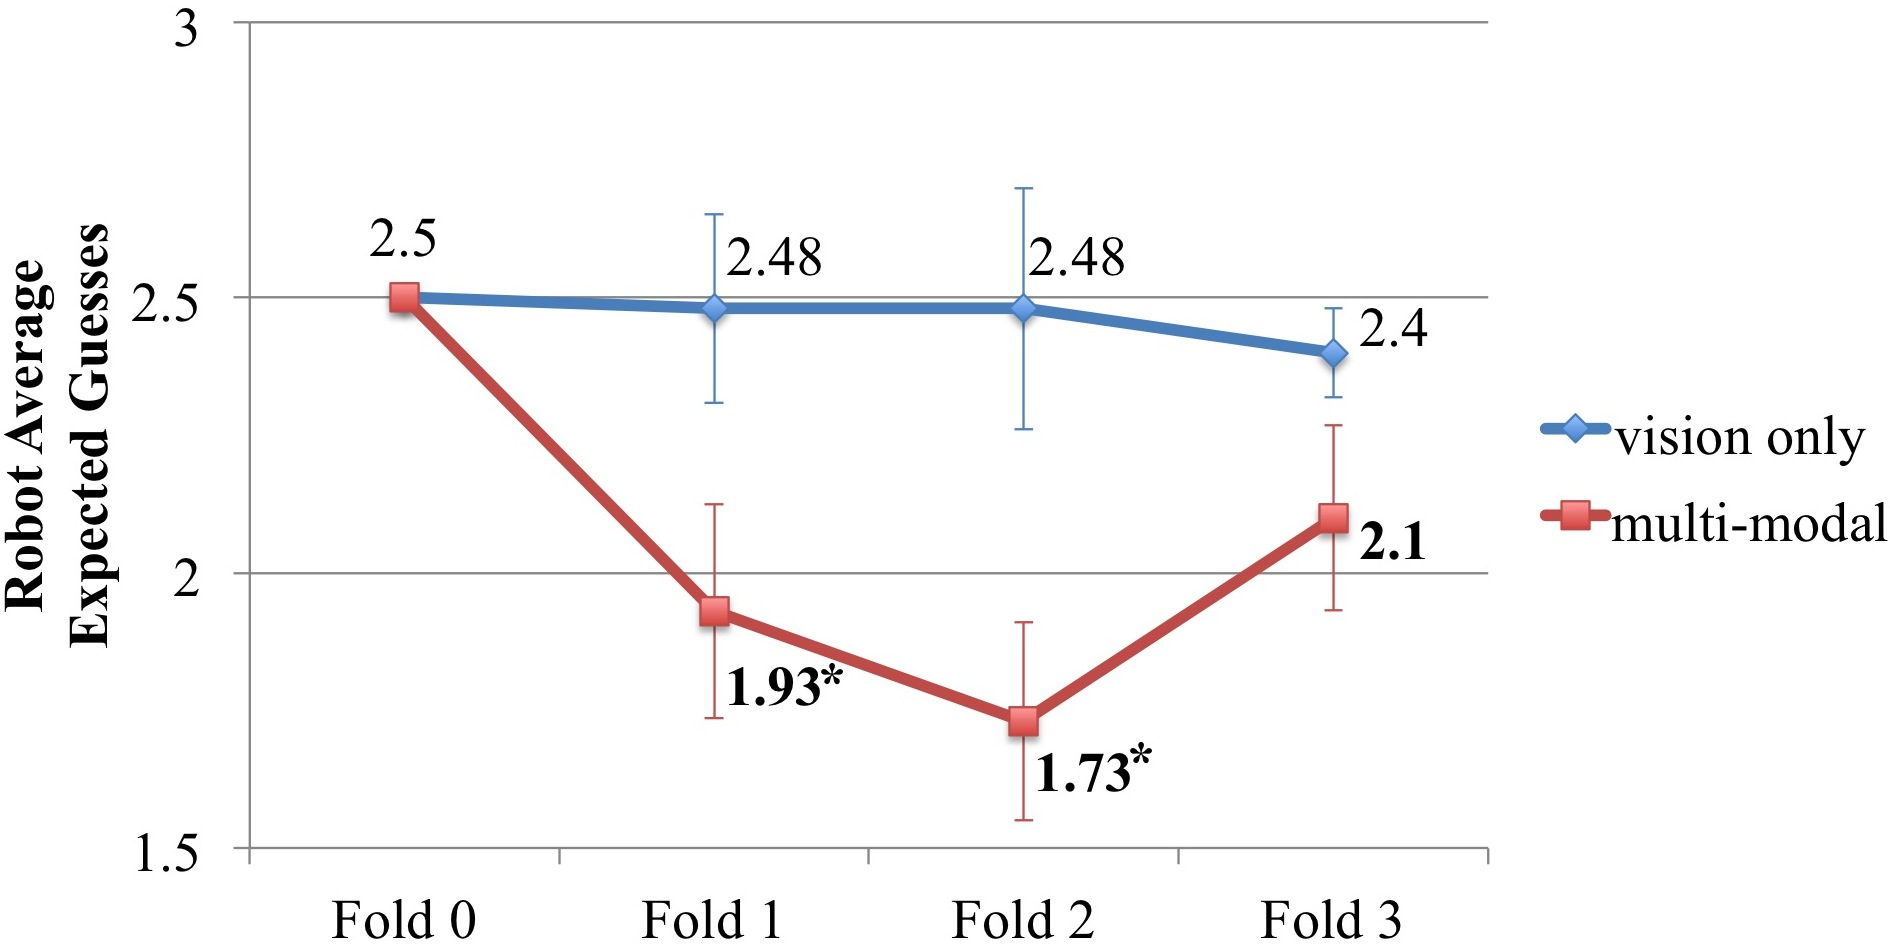
\includegraphics[width=0.5\textwidth]{figures/robot_guesses_error_bars.jpg}
\caption{Average expected number of guesses the robot made on each human turn with standard error bars shown.
\textbf{Bold}: significantly lower than the average at fold 0 with $p<0.05$ (unpaired Student's $t$-test).
\textbf{*}: significantly lower than the competing system on this fold on participant-by-participant basis with $p<0.05$ (paired Student's $t$-test).}
\label{fig:robot_guesses}
\end{figure}

\textbf{Robot guess.} Figure~\ref{fig:robot_guesses} shows the average number of robot guesses for the games in each fold. Because we had access to the scores the robot assigned each object, we calculated the {\it expected} number of robot guesses for each turn.
For example, if all 4 objects were tied for first, the expected number of robot guesses for that turn was 2.5, regardless of whether it got (un)lucky and picked the correct object (last)first.\footnote{2.5 is the expected number for 4 tied objects because the probability of picking in any order is equal, so the expected turn to get the correct object is $\frac{1+2+3+4}{4} = \frac{10}{4} = 2.5$}

After training on just one fold, our \textbf{multi-modal} approach performs statistically significantly better than the expected number of turns for guessing (the strategy for the untrained fold 0 system) for the remainder of the games.
The \textbf{vision only} system, by contrast, is never able to differentiate itself significantly from random guessing, even as more training data becomes available.
We suspect the number of objects is too small for the \textbf{vision only} system to develop decent models of many predicates, whereas \textbf{multi-modal} exploration allows that system to extract more information per object.

\textbf{Human guess.} Neither the \textbf{vision only} nor \textbf{multi-modal} system's performance improves on this metric with statistical significance as more training data is seen.
Human guesses hovered around 2.5 throughout all levels of training and sets of objects.

This result highlights the difficulty of the robot's turn in an \ispy framework, which requires not just good coverage of grounded words (as when figuring out what object the human is describing), but also high accuracy when using classifiers on new objects.
Context classifiers which had few examples could achieve confidence $\kappa=1$, making the predicates they represented more likely to be chosen to describe objects.
It is possible that the system would have performed better on this metric if the predicate scoring function $R$ additionally favored predicates with many examples.

\textbf{Predicate Agreement.} \DIFdelbegin \DIFdel{After training }\DIFdelend \DIFaddbegin \DIFadd{Training }\DIFaddend the predicate classifiers using \DIFdelbegin \DIFdel{data gathered over all folds of }\DIFdelend \DIFaddbegin \DIFadd{leave-one-out cross validation over }\DIFaddend objects, we calculated the \DIFaddbegin \DIFadd{average }\DIFaddend precision, recall, \DIFaddbegin \DIFadd{and }\DIFaddend $F_1$ \DIFdelbegin \DIFdel{, and $\kappa$ }\DIFdelend scores of each against \DIFdelbegin \DIFdel{the human labels on which they were trained}\DIFdelend \DIFaddbegin \DIFadd{human predicate labels on the held-out object}\DIFaddend .
Table~\ref{tab:predicate_results} gives these metrics for the \DIFdelbegin \DIFdel{54 predicates shared between }\DIFdelend \DIFaddbegin \DIFadd{74 predicates used by }\DIFaddend the systems.\footnote{There were \DIFdelbegin \DIFdel{129 }\DIFdelend \DIFaddbegin \DIFadd{53 }\DIFaddend predicates \DIFdelbegin \DIFdel{total }\DIFdelend \DIFaddbegin \DIFadd{shared }\DIFaddend between \DIFdelbegin \DIFdel{both }\DIFdelend \DIFaddbegin \DIFadd{the two }\DIFaddend systems.
The results in Table~\ref{tab:predicate_results} \DIFdelbegin \DIFdel{hold with significance }\DIFdelend \DIFaddbegin \DIFadd{are similar }\DIFaddend for \DIFdelbegin \DIFdel{an unsigned }\DIFdelend \DIFaddbegin \DIFadd{a paired }\DIFaddend $t$-test across \DIFdelbegin \DIFdel{all 129 }\DIFdelend \DIFaddbegin \DIFadd{these shared }\DIFaddend predicates \DIFdelbegin \DIFdel{as well, }\DIFdelend with \DIFdelbegin \DIFdel{the exception of $\kappa$ differing with only $p<0.1$}\DIFdelend \DIFaddbegin \DIFadd{slightly reduced significance}\DIFaddend .}

\begin{table}
\centering
\begin{tabular}[h]{|l|r|r|}
	\hline
	\bf Metric & \multicolumn{2}{c|}{\bf System} \\ \hline \hline
	& \bf vision only & \bf multi-modal \\ \hline
	precision & \DIFdelbeginFL \DIFdelFL{.306 }\DIFdelendFL \DIFaddbeginFL \DIFaddFL{.250 }\DIFaddendFL & \DIFdelbeginFL \DIFdelFL{.497}\DIFdelendFL \DIFaddbeginFL \DIFaddFL{.378}\DIFaddendFL \textbf{\DIFdelbeginFL \DIFdelFL{*}\DIFdelendFL \DIFaddbeginFL \DIFaddFL{+}\DIFaddendFL } \\
	recall & \DIFdelbeginFL \DIFdelFL{.340 }\DIFdelendFL \DIFaddbeginFL \DIFaddFL{.179 }\DIFaddendFL & \DIFdelbeginFL \DIFdelFL{.530}\DIFdelendFL \DIFaddbeginFL \DIFaddFL{.348}\DIFaddendFL \textbf{*} \\
	\bf $F_1$ & \DIFdelbeginFL \DIFdelFL{.317 }%DIFDELCMD < & %%%
\DIFdelFL{.498}\textbf{\DIFdelFL{*}} %DIFAUXCMD
%DIFDELCMD < \\
%DIFDELCMD < 	\bf %%%
\DIFdelFL{$\kappa$ }%DIFDELCMD < & %%%
\DIFdelFL{.105 }\DIFdelendFL \DIFaddbeginFL \DIFaddFL{.196 }\DIFaddendFL & \DIFdelbeginFL \DIFdelFL{.212}\DIFdelendFL \DIFaddbeginFL \DIFaddFL{.354}\DIFaddendFL \textbf{*} \\ \hline
\end{tabular}
\caption{\DIFdelbeginFL \DIFdelFL{Agreement metrics }\DIFdelendFL \DIFaddbeginFL \DIFaddFL{Average performance }\DIFaddendFL of predicate classifiers \DIFdelbeginFL \DIFdelFL{shared between }\DIFdelendFL \DIFaddbeginFL \DIFaddFL{used by }\DIFaddendFL the \textbf{vision only} and \textbf{multi-modal} systems \DIFaddbeginFL \DIFaddFL{in leave-one-object-out cross validation}\DIFaddendFL .
\textbf{*}: \DIFdelbeginFL \DIFdelFL{a }\DIFdelendFL significantly greater than competing system with $p<0.05$\DIFaddbeginFL \DIFaddFL{.
}\textbf{\DIFaddFL{+}}\DIFaddFL{: $p<0.1$ }\DIFaddendFL (Student's \DIFdelbeginFL \DIFdelFL{paired }\DIFdelendFL \DIFaddbeginFL \DIFaddFL{un-paired }\DIFaddendFL $t$-test).}
\label{tab:predicate_results}
\end{table}

Across the objects our robot explored, our \textbf{multi-modal} system achieves consistently better agreement with human assignments of predicates to objects than does the \textbf{vision only} system.


	\subsection{Qualitative Results}
	\label{ssec:qualitative}
We explored the predicates learned by our systems qualitatively by looking at the differences in individual predicate classifier agreements, the objects picked out by these classifiers in each system, and correlations between predicate decisions and physical properties of objects.

\textbf{When multi-modal helps.} We performed a pairwise comparison of predicates built in the \textbf{multi-modal} and \textbf{vision only} systems\DIFaddbegin \DIFadd{, again using leave-one-out cross validation over objects to measure performance}\DIFaddend .
Table~\ref{tab:predicate_examples} shows the predicates for which the difference in \DIFdelbegin \DIFdel{$\kappa$ }\DIFdelend \DIFaddbegin \DIFadd{$f_1$ }\DIFaddend between the two systems was high.

\begin{table*}
\centering
\begin{tabular}[t]{| c | c || >{\centering\arraybackslash}m{\pictablew} | >{\centering\arraybackslash}m{\pictablew} | >{\centering\arraybackslash}m{\pictablew} || >{\centering\arraybackslash}m{\pictablew} | >{\centering\arraybackslash}m{\pictablew} | >{\centering\arraybackslash}m{\pictablew} |}
	\hline
	\bf Predicate & \DIFdelbeginFL \DIFdelFL{$\kappa_{mm}-\kappa_{vo}$ }\DIFdelendFL \DIFaddbeginFL \DIFaddFL{$f_1^{mm}-f_1^{vo}$ }\DIFaddendFL & \multicolumn{3}{c||}{\bf High Confidence Positive} & \multicolumn{3}{c|}{\bf High Confidence Negative} \\ \hline \hline
	\multicolumn{2}{|c|}{} & \multicolumn{6}{c|}{\bf multi-modal system} \\ \hline
	can & \DIFdelbeginFL \DIFdelFL{1 }%DIFDELCMD < & 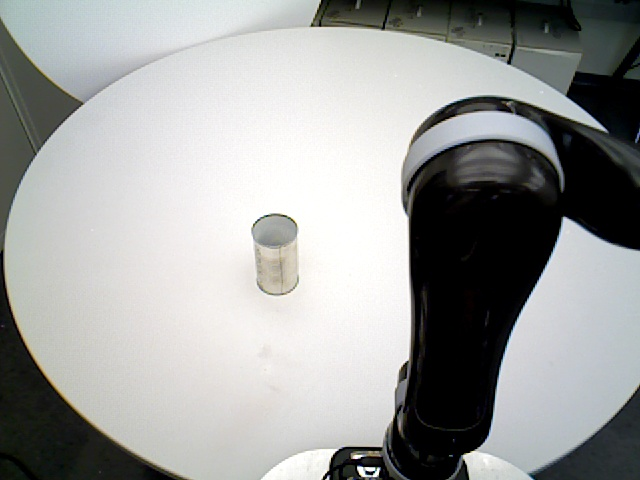
\includegraphics[scale=\examplepicsize]{figures/objects/9.JPG} %%%
\DIFdelendFL \DIFaddbeginFL \DIFaddFL{0.857 }\DIFaddendFL & 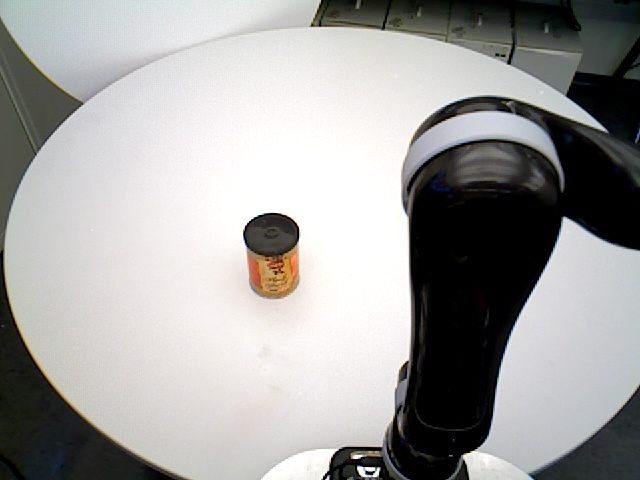
\includegraphics[scale=\examplepicsize]{figures/objects/3.JPG} & \DIFaddbeginFL 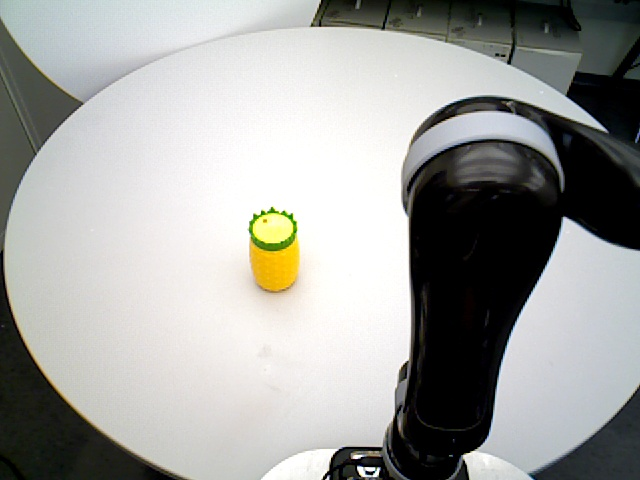
\includegraphics[scale=\examplepicsize]{figures/objects/5.JPG} & \DIFaddendFL 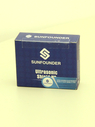
\includegraphics[scale=\examplepicsize]{figures/objects/6.JPG} & \DIFdelbeginFL %DIFDELCMD < 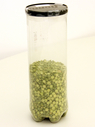
\includegraphics[scale=\examplepicsize]{figures/objects/28.JPG} %%%
\DIFdelendFL \DIFaddbeginFL 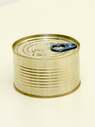
\includegraphics[scale=\examplepicsize]{figures/objects/30.JPG} \DIFaddendFL & \DIFdelbeginFL %DIFDELCMD < 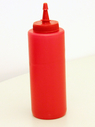
\includegraphics[scale=\examplepicsize]{figures/objects/21.JPG} %%%
\DIFdelendFL \DIFaddbeginFL 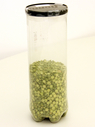
\includegraphics[scale=\examplepicsize]{figures/objects/28.JPG} \DIFaddendFL & \DIFdelbeginFL %DIFDELCMD < 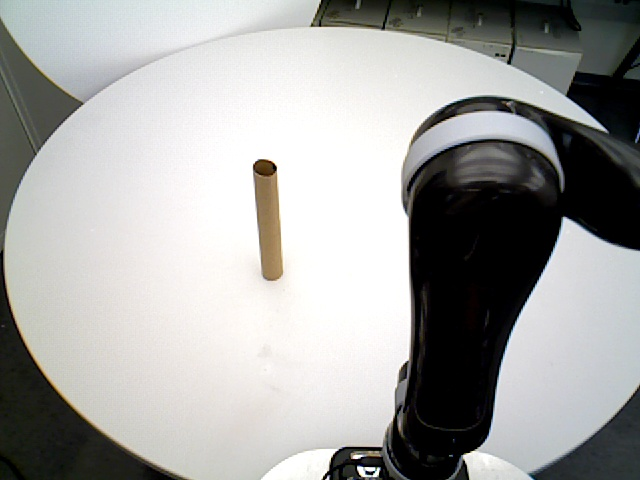
\includegraphics[scale=\examplepicsize]{figures/objects/4.JPG}%%%
\DIFdelendFL \DIFaddbeginFL 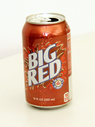
\includegraphics[scale=\examplepicsize]{figures/objects/15.JPG}\DIFaddendFL \\ \hline
	\DIFdelbeginFL \DIFdelFL{tub }\DIFdelendFL \DIFaddbeginFL \DIFaddFL{tall }\DIFaddendFL & \DIFdelbeginFL \DIFdelFL{1 }\DIFdelendFL \DIFaddbeginFL \DIFaddFL{0.516 }\DIFaddendFL & \DIFdelbeginFL %DIFDELCMD < 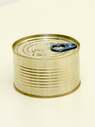
\includegraphics[scale=\examplepicsize]{figures/objects/30.JPG} %%%
\DIFdelendFL \DIFaddbeginFL 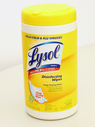
\includegraphics[scale=\examplepicsize]{figures/objects/22.JPG} \DIFaddendFL & \DIFdelbeginFL %DIFDELCMD < 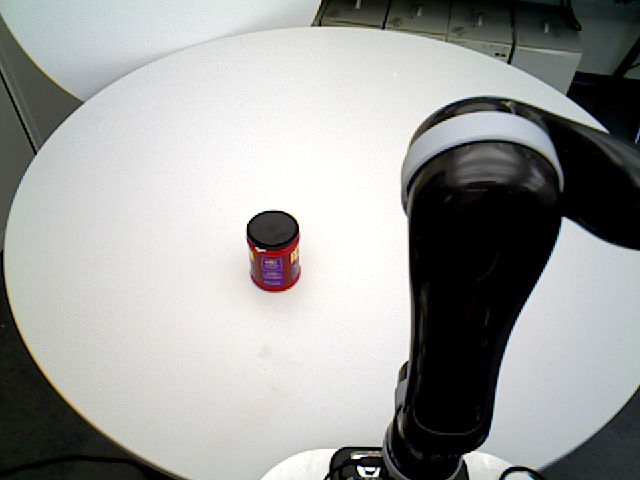
\includegraphics[scale=\examplepicsize]{figures/objects/10.JPG} %%%
\DIFdelendFL \DIFaddbeginFL 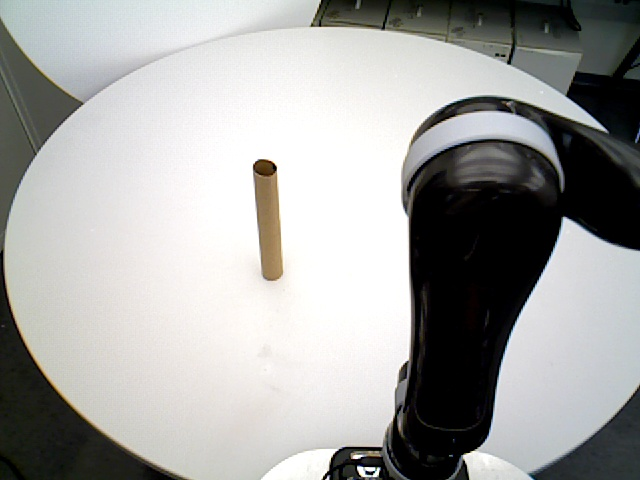
\includegraphics[scale=\examplepicsize]{figures/objects/4.JPG} \DIFaddendFL & \DIFdelbeginFL %DIFDELCMD < 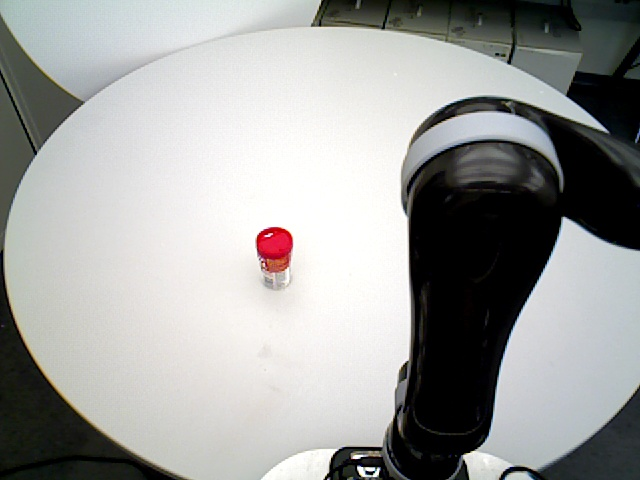
\includegraphics[scale=\examplepicsize]{figures/objects/11.JPG} %%%
\DIFdelendFL \DIFaddbeginFL 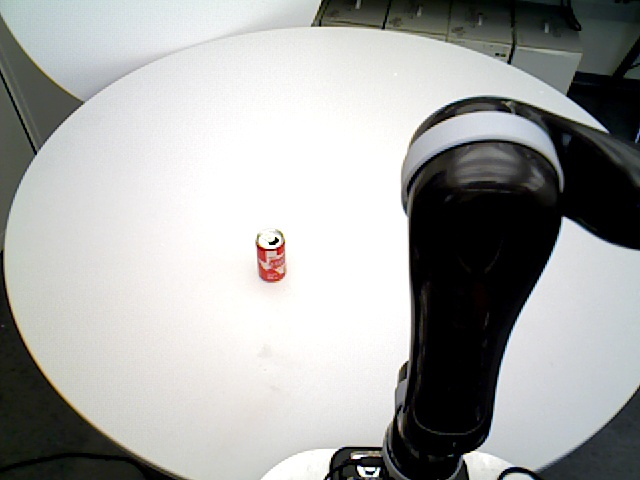
\includegraphics[scale=\examplepicsize]{figures/objects/27.JPG} \DIFaddendFL & \DIFdelbeginFL %DIFDELCMD < 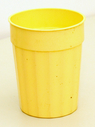
\includegraphics[scale=\examplepicsize]{figures/objects/14.JPG} %%%
\DIFdelendFL \DIFaddbeginFL 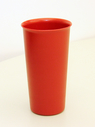
\includegraphics[scale=\examplepicsize]{figures/objects/7.JPG} \DIFaddendFL & \DIFdelbeginFL %DIFDELCMD < 
\includegraphics[scale=\examplepicsize]{figures/objects/2.JPG} %%%
\DIFdelendFL \DIFaddbeginFL 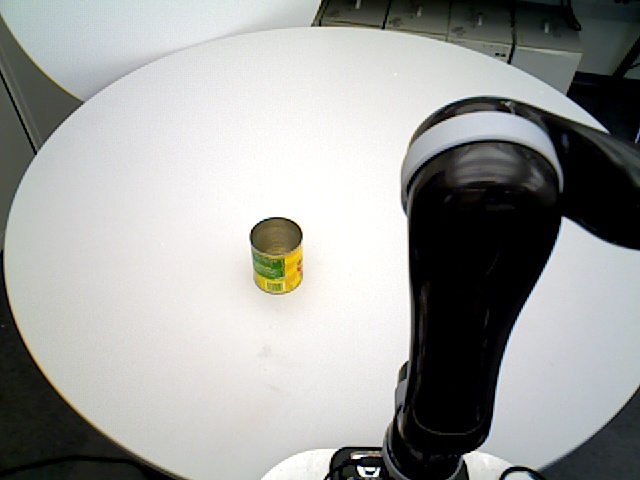
\includegraphics[scale=\examplepicsize]{figures/objects/12.JPG} \DIFaddendFL & \DIFdelbeginFL %DIFDELCMD < 
\includegraphics[scale=\examplepicsize]{figures/objects/18.JPG}%%%
\DIFdelendFL \DIFaddbeginFL 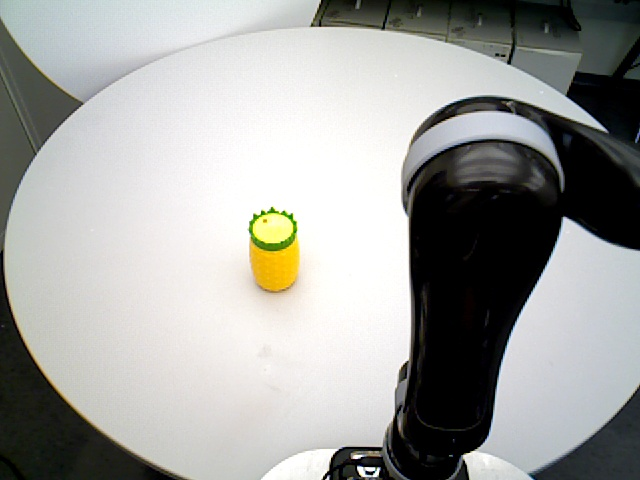
\includegraphics[scale=\examplepicsize]{figures/objects/5.JPG}\DIFaddendFL \\ \hline
	\DIFdelbeginFL \DIFdelFL{empty }\DIFdelendFL \DIFaddbeginFL \DIFaddFL{half-full }\DIFaddendFL & \DIFdelbeginFL \DIFdelFL{.637 }\DIFdelendFL \DIFaddbeginFL \DIFaddFL{.462 }\DIFaddendFL & \DIFdelbeginFL %DIFDELCMD < 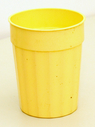
\includegraphics[scale=\examplepicsize]{figures/objects/14.JPG} %%%
\DIFdelendFL \DIFaddbeginFL 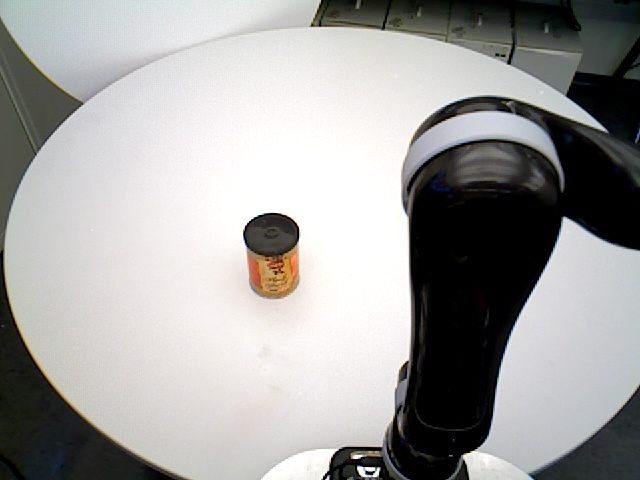
\includegraphics[scale=\examplepicsize]{figures/objects/3.JPG} \DIFaddendFL & \DIFdelbeginFL %DIFDELCMD < 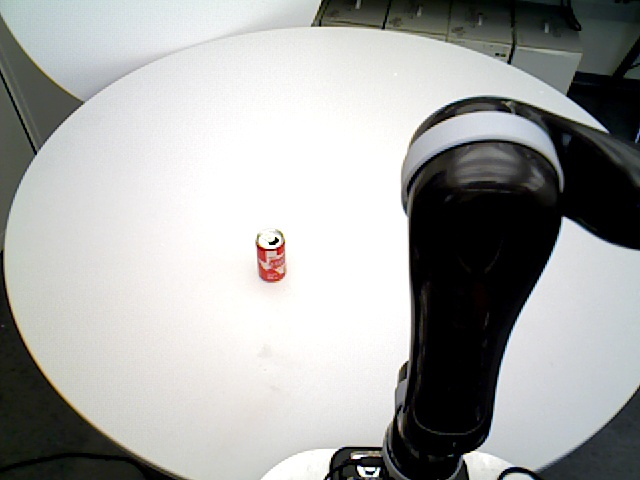
\includegraphics[scale=\examplepicsize]{figures/objects/27.JPG} %%%
\DIFdelendFL \DIFaddbeginFL 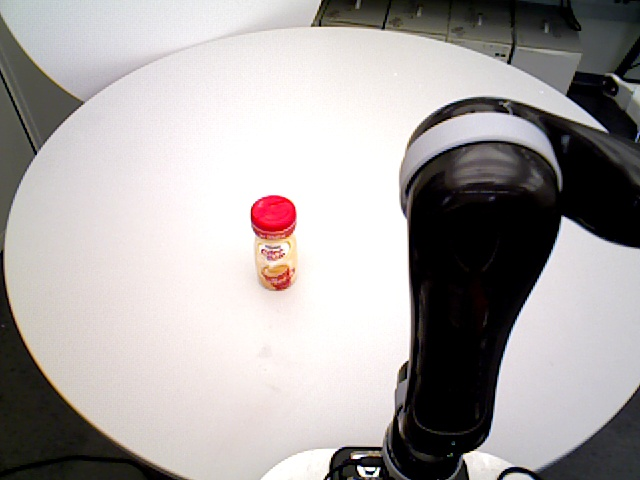
\includegraphics[scale=\examplepicsize]{figures/objects/17.JPG} \DIFaddendFL & \DIFdelbeginFL %DIFDELCMD < 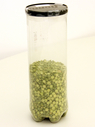
\includegraphics[scale=\examplepicsize]{figures/objects/28.JPG} %%%
\DIFdelendFL \DIFaddbeginFL 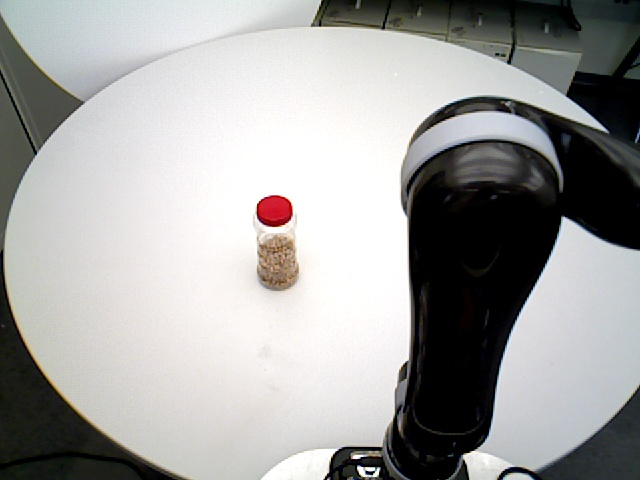
\includegraphics[scale=\examplepicsize]{figures/objects/23.JPG} \DIFaddendFL & \DIFdelbeginFL %DIFDELCMD < 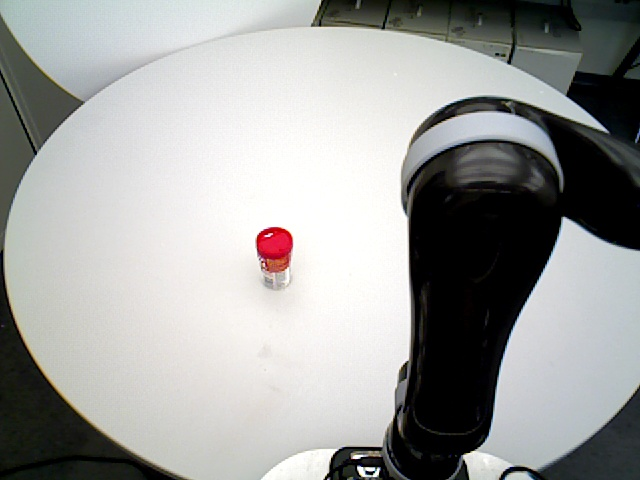
\includegraphics[scale=\examplepicsize]{figures/objects/11.JPG} %%%
\DIFdelendFL \DIFaddbeginFL 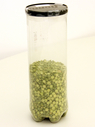
\includegraphics[scale=\examplepicsize]{figures/objects/28.JPG} \DIFaddendFL & \DIFdelbeginFL %DIFDELCMD < 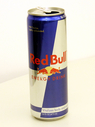
\includegraphics[scale=\examplepicsize]{figures/objects/31.JPG} %%%
\DIFdelendFL \DIFaddbeginFL 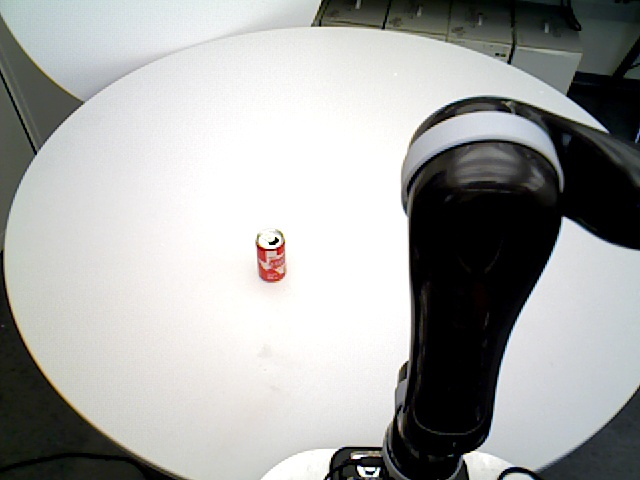
\includegraphics[scale=\examplepicsize]{figures/objects/27.JPG} \DIFaddendFL & \DIFdelbeginFL %DIFDELCMD < 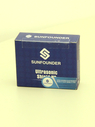
\includegraphics[scale=\examplepicsize]{figures/objects/6.JPG}%%%
\DIFdelendFL \DIFaddbeginFL 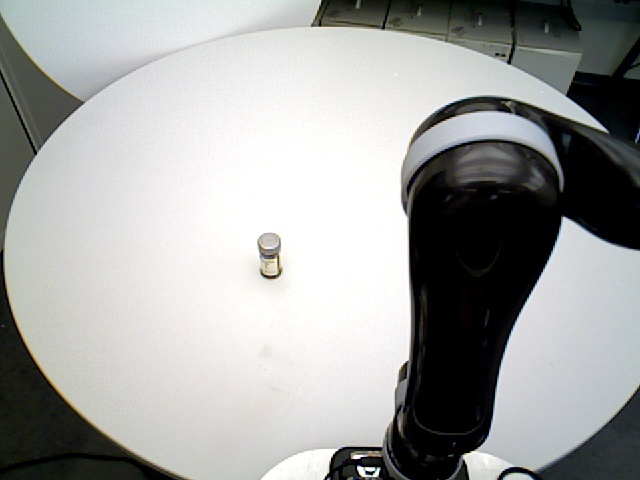
\includegraphics[scale=\examplepicsize]{figures/objects/26.JPG}\DIFaddendFL \\ \hline
	\DIFdelbeginFL \DIFdelFL{tall }\DIFdelendFL \DIFaddbeginFL \DIFaddFL{yellow }\DIFaddendFL & \DIFdelbeginFL \DIFdelFL{.566 }\DIFdelendFL \DIFaddbeginFL \DIFaddFL{.312 }\DIFaddendFL & \DIFdelbeginFL %DIFDELCMD < 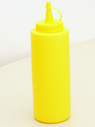
\includegraphics[scale=\examplepicsize]{figures/objects/19.JPG} %%%
\DIFdelendFL \DIFaddbeginFL 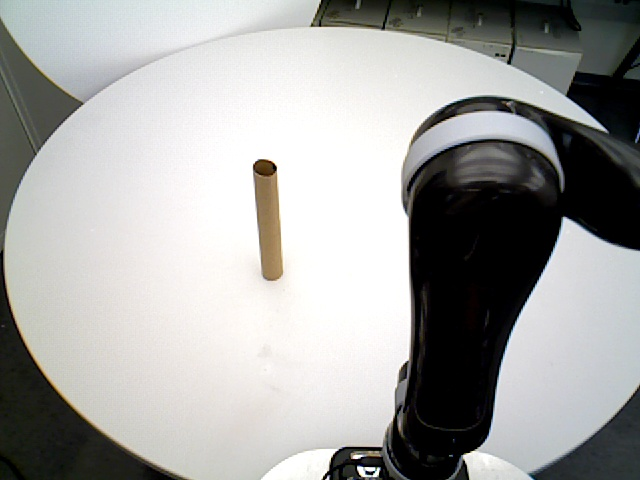
\includegraphics[scale=\examplepicsize]{figures/objects/4.JPG} \DIFaddendFL & \DIFdelbeginFL %DIFDELCMD < 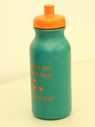
\includegraphics[scale=\examplepicsize]{figures/objects/24.JPG} %%%
\DIFdelendFL \DIFaddbeginFL 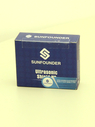
\includegraphics[scale=\examplepicsize]{figures/objects/6.JPG} \DIFaddendFL & \DIFdelbeginFL %DIFDELCMD < 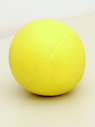
\includegraphics[scale=\examplepicsize]{figures/objects/25.JPG} %%%
\DIFdelendFL \DIFaddbeginFL 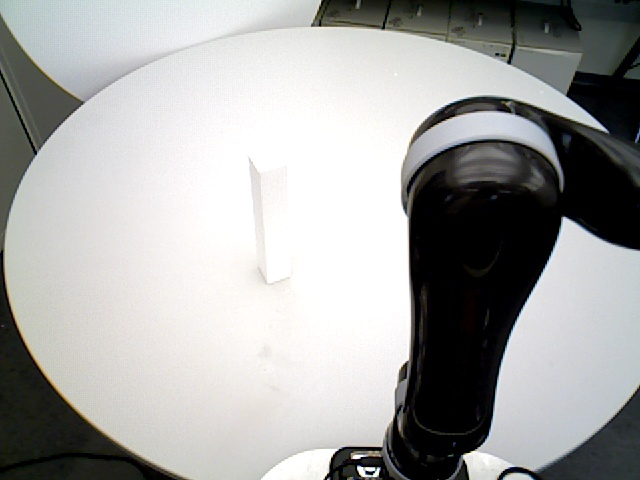
\includegraphics[scale=\examplepicsize]{figures/objects/29.JPG} \DIFaddendFL & \DIFdelbeginFL %DIFDELCMD < \includegraphics[scale=\examplepicsize]{figures/objects/15.JPG} %%%
\DIFdelendFL \DIFaddbeginFL \includegraphics[scale=\examplepicsize]{figures/objects/18.JPG} \DIFaddendFL & \DIFdelbeginFL %DIFDELCMD < \includegraphics[scale=\examplepicsize]{figures/objects/26.JPG} %%%
\DIFdelendFL \DIFaddbeginFL \includegraphics[scale=\examplepicsize]{figures/objects/23.JPG} \DIFaddendFL & \DIFdelbeginFL %DIFDELCMD < \includegraphics[scale=\examplepicsize]{figures/objects/7.JPG}%%%
\DIFdelendFL \DIFaddbeginFL \includegraphics[scale=\examplepicsize]{figures/objects/17.JPG}\DIFaddendFL \\ \hline
	\multicolumn{2}{|c|}{} & \multicolumn{6}{c|}{\bf vision only system} \\ \hline
	\DIFdelbeginFL \DIFdelFL{small }%DIFDELCMD < & %%%
\DIFdelFL{-.25 }%DIFDELCMD < & \includegraphics[scale=\examplepicsize]{figures/objects/2.JPG} & \includegraphics[scale=\examplepicsize]{figures/objects/7.JPG} & \includegraphics[scale=\examplepicsize]{figures/objects/13.JPG} & \includegraphics[scale=\examplepicsize]{figures/objects/32.JPG} & \includegraphics[scale=\examplepicsize]{figures/objects/31.JPG} %%%
\DIFdelendFL \DIFaddbeginFL \DIFaddFL{pink }\DIFaddendFL & \DIFdelbeginFL %DIFDELCMD < \includegraphics[scale=\examplepicsize]{figures/objects/25.JPG}\\ \hline
%DIFDELCMD < 	%%%
\DIFdelFL{red }\DIFdelendFL \DIFaddbeginFL \DIFaddFL{-.3 }\DIFaddendFL & \DIFdelbeginFL \DIFdelFL{-.663 }\DIFdelendFL \DIFaddbeginFL \includegraphics[scale=\examplepicsize]{figures/objects/11.JPG} \DIFaddendFL & \DIFdelbeginFL %DIFDELCMD < \includegraphics[scale=\examplepicsize]{figures/objects/8.JPG} %%%
\DIFdelendFL \DIFaddbeginFL \includegraphics[scale=\examplepicsize]{figures/objects/23.JPG} \DIFaddendFL & \includegraphics[scale=\examplepicsize]{figures/objects/10.JPG} & \DIFdelbeginFL %DIFDELCMD < \includegraphics[scale=\examplepicsize]{figures/objects/14.JPG} & \includegraphics[scale=\examplepicsize]{figures/objects/12.JPG} & \includegraphics[scale=\examplepicsize]{figures/objects/5.JPG} & \includegraphics[scale=\examplepicsize]{figures/objects/3.JPG}\\ \hline
%DIFDELCMD < 	%%%
\DIFdelFL{yellow }%DIFDELCMD < & %%%
\DIFdelFL{-1 }%DIFDELCMD < & \includegraphics[scale=\examplepicsize]{figures/objects/12.JPG} & \includegraphics[scale=\examplepicsize]{figures/objects/20.JPG} & \includegraphics[scale=\examplepicsize]{figures/objects/25.JPG} & \includegraphics[scale=\examplepicsize]{figures/objects/1.JPG} %%%
\DIFdelendFL \DIFaddbeginFL \includegraphics[scale=\examplepicsize]{figures/objects/8.JPG} \DIFaddendFL & \DIFdelbeginFL %DIFDELCMD < \includegraphics[scale=\examplepicsize]{figures/objects/4.JPG} %%%
\DIFdelendFL \DIFaddbeginFL \includegraphics[scale=\examplepicsize]{figures/objects/2.JPG} \DIFaddendFL & \DIFdelbeginFL %DIFDELCMD < \includegraphics[scale=\examplepicsize]{figures/objects/17.JPG}%%%
\DIFdelendFL \DIFaddbeginFL \includegraphics[scale=\examplepicsize]{figures/objects/27.JPG}\DIFaddendFL \\ \hline
\end{tabular}
\caption{Predicates for which the difference \DIFdelbeginFL \DIFdelFL{$|\kappa_{mm}-\kappa_{vo}|$ }\DIFdelendFL \DIFaddbeginFL \DIFaddFL{$|f_1^{mm}-f_1^{vo}|$ }\DIFaddendFL between the \textbf{multi-modal} (mm) and \textbf{vision only} (vo) systems was greater than \DIFdelbeginFL \DIFdelFL{$0.5$ and }\DIFdelendFL \DIFaddbeginFL \DIFaddFL{or equal to $0.3$, }\DIFaddendFL both systems had at least $10$ objects with labels for that predicate on which to train\DIFaddbeginFL \DIFaddFL{, and the system with the worse $f_1$ had at most 5 fewer objects with labels on which to train (to avoid rewarding a system just for having more training labels)}\DIFaddendFL . The highest- and lowest-confidence objects for each predicate are shown. The top rows (\DIFdelbeginFL \DIFdelFL{$\kappa_{mm}-\kappa_{vo}>0$}\DIFdelendFL \DIFaddbeginFL \DIFaddFL{$f_1^{mm}-f_1^{vo}>0$}\DIFaddendFL ) are decisions from the \textbf{multi-modal} system, the bottom rows the \textbf{vision only} system.}
\label{tab:predicate_examples}
\end{table*}

The \textbf{multi-modal} system \DIFdelbegin \DIFdel{achieves total agreement with human labels for ``can'' and ``tub;''
whereas the }\textbf{\DIFdel{vision only}} %DIFAUXCMD
\DIFdel{system classified all objects as not having these properties, giving $\kappa=0$ (the }\textbf{\DIFdel{multi-modal}} %DIFAUXCMD
\DIFdel{system did something comparable for ``yellow'').
We note that ``can'' and ``tub'' are cases of category recognition, for which visual data is certainly helpful, but the non-visual attributes of an object may also contribute (e.g. cans are light, tubs are heavy).
In contrast, ``yellow'' is a color word for which only visual properties are relevant, and the additional noise from other features were enough to confuse the }\textbf{\DIFdel{multi-modal}} %DIFAUXCMD
\DIFdel{approach.
}%DIFDELCMD < 

%DIFDELCMD < %%%
\DIFdel{The predicates ``empty}\DIFdelend \DIFaddbegin \DIFadd{does well on the predicates ``tall}\DIFaddend '' and ``\DIFdelbegin \DIFdel{tall'' }\DIFdelend \DIFaddbegin \DIFadd{half-full'' which }\DIFaddend have non-visual interpretations.
\DIFdelbegin \DIFdel{An empty object will be light, while }\DIFdelend \DIFaddbegin \DIFadd{A }\DIFaddend a tall object will exert force earlier against an arm pressing down on it\DIFaddbegin \DIFadd{, while half-full object will be lighter than a full one and heavier than an empty one}\DIFaddend .
The color predicate ``\DIFdelbegin \DIFdel{red'' follows the same reasoning as ``yellow'' , where non-visual information can serve only to confuse a }\DIFdelend \DIFaddbegin \DIFadd{pink'' seems to confuse the }\DIFaddend multi-modal grounding system \DIFdelbegin \DIFdel{.
The correlation results in Table~\ref{tab:predicate_correlations} indicate that the }\textbf{\DIFdel{vision only}} %DIFAUXCMD
\DIFdel{system learned to associate ``small''with decreased object width, while the }\textbf{\DIFdel{multi-modal}} %DIFAUXCMD
\DIFdel{systemwas again confused by additional }\DIFdelend \DIFaddbegin \DIFadd{using }\DIFaddend non-visual \DIFdelbegin \DIFdel{information}\DIFdelend \DIFaddbegin \DIFadd{information for this purely visual predicate.
This doesn't hold for ``yellow'', though the classifiers for ``yellow'' never became particularly good for either system.
For example, two of the three most confident objects in the multi-modal setting are in fact not yellow}\DIFaddend .

\textbf{Correlations to \DIFdelbegin \DIFdel{objective measures}\DIFdelend \DIFaddbegin \DIFadd{physical properties}\DIFaddend .} To validate whether the systems are learning non-visual properties of objects, for every predicate we calculated the Pearson's correlation $r$ between its decision on each object and that object's measured weight, height, and width. 
\DIFdelbegin \DIFdel{Table~\ref{tab:predicate_correlations} gives the correlations with both high coefficient $r$ and high statistical confidence}\DIFdelend \DIFaddbegin \DIFadd{As before, the decisions were made on held-out objects in leave-one-out cross validation.
We found predicates for which $r>0.5$ with $p<0.05$ when the system had at least $10$ objects with labels for the predicate on which to train}\DIFaddend .

\DIFdelbegin %DIFDELCMD < \begin{table}
%DIFDELCMD < \centering
%DIFDELCMD < \begin{tabular}[h]{|l|r|r|}
%DIFDELCMD < 	\hline
%DIFDELCMD < 	\bf %%%
\DIFdel{Property }%DIFDELCMD < & \bf %%%
\DIFdel{multi-modal }%DIFDELCMD < & \bf %%%
\DIFdel{vision only }%DIFDELCMD < \\ \hline \hline
%DIFDELCMD < 	& \multicolumn{2}{c|}{\bf Believable} \\ \hline
%DIFDELCMD < 	\bf %%%
\DIFdel{height }%DIFDELCMD < & %%%
\DIFdel{tall (.739) }%DIFDELCMD < & %%%
\DIFdel{heavy (.729) }%DIFDELCMD < \\ \hline
%DIFDELCMD < 	\bf %%%
\DIFdel{width }%DIFDELCMD < & %%%
\DIFdel{fat (.509) }%DIFDELCMD < & %%%
\DIFdel{small (-.525) }%DIFDELCMD < \\ \hline
%DIFDELCMD < 	\bf %%%
\DIFdel{weight }%DIFDELCMD < & %%%
\DIFdel{empty (-.771) }%DIFDELCMD < & \\ \hline \hline
%DIFDELCMD < 	& \multicolumn{2}{c|}{\bf Likely spurious} \\ \hline
%DIFDELCMD < 	\bf %%%
\DIFdel{width }%DIFDELCMD < & & %%%
\DIFdel{rattles }%DIFDELCMD < \\ \hline
%DIFDELCMD < 	& %%%
\DIFdel{water, blue, }%DIFDELCMD < & \\
%DIFDELCMD < 	\bf %%%
\DIFdel{weight }%DIFDELCMD < & %%%
\DIFdel{silver, liquid, }%DIFDELCMD < & \\ 
%DIFDELCMD < 	& %%%
\DIFdel{gray, red, yellow }%DIFDELCMD < & \\ \hline
%DIFDELCMD < \end{tabular}
%DIFDELCMD < %%%
%DIFDELCMD < \caption{%
{%DIFAUXCMD
\DIFdel{Predicates and associated Pearson's correlation coefficient $r$ between systems' object decisions and physical object properties.
Shown here are predicates for which $r>0.5$ with $p<0.05$ and the system had at least $10$ objects with labels for the predicate on which to train.}}
%DIFAUXCMD
%DIFDELCMD < \label{tab:predicate_correlations}
%DIFDELCMD < \end{table}
%DIFDELCMD < 

%DIFDELCMD < %%%
\DIFdelend The \textbf{vision only} system \DIFdelbegin \DIFdel{seems able to ground ``heavy'' in height and ``small'' in width.
The system can sense these physical properties through the vision featuresassociated with the pointcloud}\DIFdelend \DIFaddbegin \DIFadd{led to no predicates correlated against these physical object features}\DIFaddend .

The \textbf{multi-modal} system learned to ground predicates which correlate well to \DIFdelbegin \DIFdel{each of the physical dimensions along which we measured objects}\DIFdelend \DIFaddbegin \DIFadd{objects' height and weight}\DIFaddend .
The ``tall'' predicate correlates with objects that are higher \DIFdelbegin \DIFdel{, ``fat'' }\DIFdelend \DIFaddbegin \DIFadd{($r=.521$), ``small'' ($r=-.665$) correlates }\DIFaddend with objects that are \DIFdelbegin \DIFdel{wider}\DIFdelend \DIFaddbegin \DIFadd{lighter}\DIFaddend , and ``\DIFdelbegin \DIFdel{empty'' }\DIFdelend \DIFaddbegin \DIFadd{water'' ($r=.814$) correlates }\DIFaddend with objects that are \DIFdelbegin \DIFdel{lighter}\DIFdelend \DIFaddbegin \DIFadd{heavier.
The latter is likely from objects described as ``water bottle'', which, in our dataset, are mostly filled either half-way or totally and thus heavier.
There is also a spurious correlation between ``blue'' and weight ($r=.549$)}\DIFaddend .
This highlights the value of multi-modal grounding, since words like ``\DIFdelbegin \DIFdel{empty}\DIFdelend \DIFaddbegin \DIFadd{half-full}\DIFaddend '' cannot be evaluated with vision alone when dealing with closed containers that have unobservable contents.


\section{Conclusion}
\label{sec:conclusion}
We expand past work on grounding natural language in robot sensory perception by going beyond vision and exploring haptic, auditory, and proprioceptive robot senses.
We compare a vision only grounding system to one that uses these additional senses by employing an embodied robot playing \ispy with many human users.
To our knowledge, ours is the first robotic system to perform natural language grounding using multi-modal sensory perception through natural interaction with human users.

We demonstrate quantitatively, through the number of turns the robot needs to guess objects described by humans, as well as through agreement with humans on language predicate labels for objects, that our multi-modal framework learns more effective lexical groundings than one using vision alone.
We also explore the learned groundings qualitatively, showing words for which non-visual information helps most as well as when non-visual properties of objects correlate with learned meanings (e.g. ``\DIFdelbegin \DIFdel{empty'' correlate }\DIFdelend \DIFaddbegin \DIFadd{small'' correlates }\DIFaddend negatively with object weight).

In the future, we would like to use one-class classification methods to remove the need for a follow-up dialog asking about particular predicates applied to an object to gather negative labels.
Additionally, we would like to detect polysemy for predicates whose meanings vary across sensory modalities.
For example, the word ``light'' can refer to weight or color.
Our current system fails to distinguish these senses, while human participants intermix them.
\DIFaddbegin \DIFadd{Additionally, in our current system, the robot needs to explore objects in advance using all of its behaviors.
However, for purely visual predicates like ``pink'' and other colors, only the }{\it \DIFadd{look}} \DIFadd{behavior is necessary to determine whether an object has the property.
We will work towards an exploration system that uses its learned knowledge of predicates from a game such as }\ispy \DIFadd{to determine the properties of a novel object while attempting to use as few exploratory behaviors as necessary.
}\DIFaddend 

%DIF <  \section*{Acknowledgments}
\DIFaddbegin \section*{\DIFadd{Acknowledgments}}

\DIFadd{We would like to thank our anonymous reviewers for their feedback and insights, our many participants for their time, and Subhashini Venugopalan for her help in engineering deep visual feature extraction. This work is supported by a National Science Foundation Graduate Research Fellowship to the first author. A portion of this work has taken place in the Learning Agents Research Group (LARG) at UT Austin. LARG research is supported in part by NSF (CNS-1330072, CNS-1305287), ONR (21C184-01), and AFOSR (FA8750-14-1-0070, FA9550-14-1-0087).
}\DIFaddend 

%% The file named.bst is a bibliography style file for BibTeX 0.99c
\DIFdelbegin %DIFDELCMD < \clearpage
%DIFDELCMD < %%%
\DIFdelend \bibliographystyle{named}
\bibliography{/u/ml/bib/lunar,/u/jesse/local}

\end{document}
